\documentclass[a4paper,12pt]{article}

\usepackage[russian]{babel}
\usepackage{cmap}
\usepackage[utf8]{inputenc}
\usepackage[usenames]{color}
\usepackage{tabularray}
\usepackage{xcolor}
\usepackage{graphicx} 
\usepackage{subfigure}
\usepackage{subcaption}

\usepackage[unicode]{hyperref}
\hypersetup{
	colorlinks,
	citecolor=black,
	filecolor=black,
	linkcolor=blue,
	urlcolor=black
}

\usepackage{geometry}
\geometry{left=2.5cm, right=1.5cm, top=2cm, bottom=2cm}

\usepackage{enumitem}
\def\labelitemi{—}
\setlist{nolistsep}

\title{\textbf{Категориальные группировки и агрегации данных об отливках в управлении качеством производства литых автомобильных деталей}}
\author{И. П. Фрелих, В. Г. Мосин\\
\small Самарский государственный технический университет (СамГТУ), Самара, Россия}
\date{}

\begin{document}
	\maketitle
	
	\abstract{\noindent В статье исследуются методы многомерной агрегации и комбинаторного перебора категориальных данных для выявления скрытых синергетических дефектов литья в автомобилестроении. На производственной выборке из 5 000 отливок доказан информационный изоморфизм факторов плавки и партии, а также локализован устойчивый очаг брака (до 24,16\%) в подгруппе «Смена 3 $\times$ Пресс-форма 9». Проведен параметрический анализ технологических сдвигов и предложен превентивный алгоритм управления качеством CAPA/EWS.}

	\tableofcontents

	\section{Введение}
	Современные литейные производства в автомобилестроении функционируют в условиях жестких требований к бездефектности ответственных узлов (блоков цилиндров, суппортов, корпусов трансмиссий). Традиционный статистический контроль процессов (SPC) на основе одномерных карт Шухарта часто оказывается неэффективным при выявлении сложных многофакторных несоответствий, когда каждый технологический параметр в отдельности находится в пределах установленного поля допуска ($\pm 3\sigma$), но их нелинейная комбинация приводит к браку.

	\section{Описание данных и постановка задачи}
	В качестве объекта исследования выступает производственный массив данных литейного цеха, включающий 5 000 последовательных отливок по 18 параметрам:
	\begin{itemize}
		\item \textbf{Категориальные факторы:} номер смены (\texttt{shift}: 1, 2, 3), номер пресс-формы (\texttt{mold\_id}: 1--12), номер плавки (\texttt{melting\_id}: 1--40), код партии (\texttt{batch\_code}: B001--B040).
		\item \textbf{Технологические параметры:} температура заливки расплава ({\text{pour}}$, \circ), скорость охлаждения в форме ({\text{cool}}$, K/мин), время выдержки ($\tau_{\text{hold}}$, мин), газосодержание расплава ({\text{gas}}$, ppm).
		\item \textbf{Метрики качества и индикатор брака:} масса, твердость по Бринеллю, пористость, амплитуда УЗ-сигнала и бинарный флаг годности (\texttt{is\_defect} $\in \{0, 1\}$).
	\end{itemize}
	Базовый уровень брака по выборке составляет {\text{base}} = 8{,}56\%$ (428 дефектных отливок).

	\section{Факторный и комбинаторный анализ}
	
	\subsection{Информационный изоморфизм}
	Оценка взаимной информации между кодом партии и номером плавки показала строгое взаимно-однозначное соответствие:
	
	I(\text{melting\_id}; \text{batch\_code}) = H(\text{batch\_code}) = 3{,}689\text{ бит}.
	
	Это позволило редуцировать исходное 4-мерное пространство объемом 57 600 состояний до 3D-матрицы объемом 1 440 ячеек.

	\subsection{Однофакторный скрининг}
	Проверка гипотезы об однородности долей брака критерием $\chi^2$ Пирсона показала:
	\begin{itemize}
		\item По смене (\texttt{shift}): $\chi^2 = 4{,}07$,  = 0{,}131$ (изолированное влияние смены статистически незначимо).
		\item По пресс-формам (\texttt{mold\_id}): $\chi^2 = 23{,}28$,  = 0{,}016$ (различия высокозначимы; форма № 9 демонстрирует повышенный брак 13,97\%).
	\end{itemize}

	\subsection{Двухфакторный анализ и синергия брака}
	Анализ сопряженности факторов «Смена $\times$ Форма» выявил резкую нелинейность ($\chi^2 = 72{,}39$,  = 0{,}00021$). В дневную смену № 2 пресс-форма № 9 обеспечивает нормативный уровень брака 7,10\%, тогда как в ночную смену № 3 уровень брака достигает критических \textbf{24,16\%} (относительный риск  = 2{,}99$,  = 4{,}67 \cdot 10^{-12}$).

	\begin{figure}[!h]
		\centering
		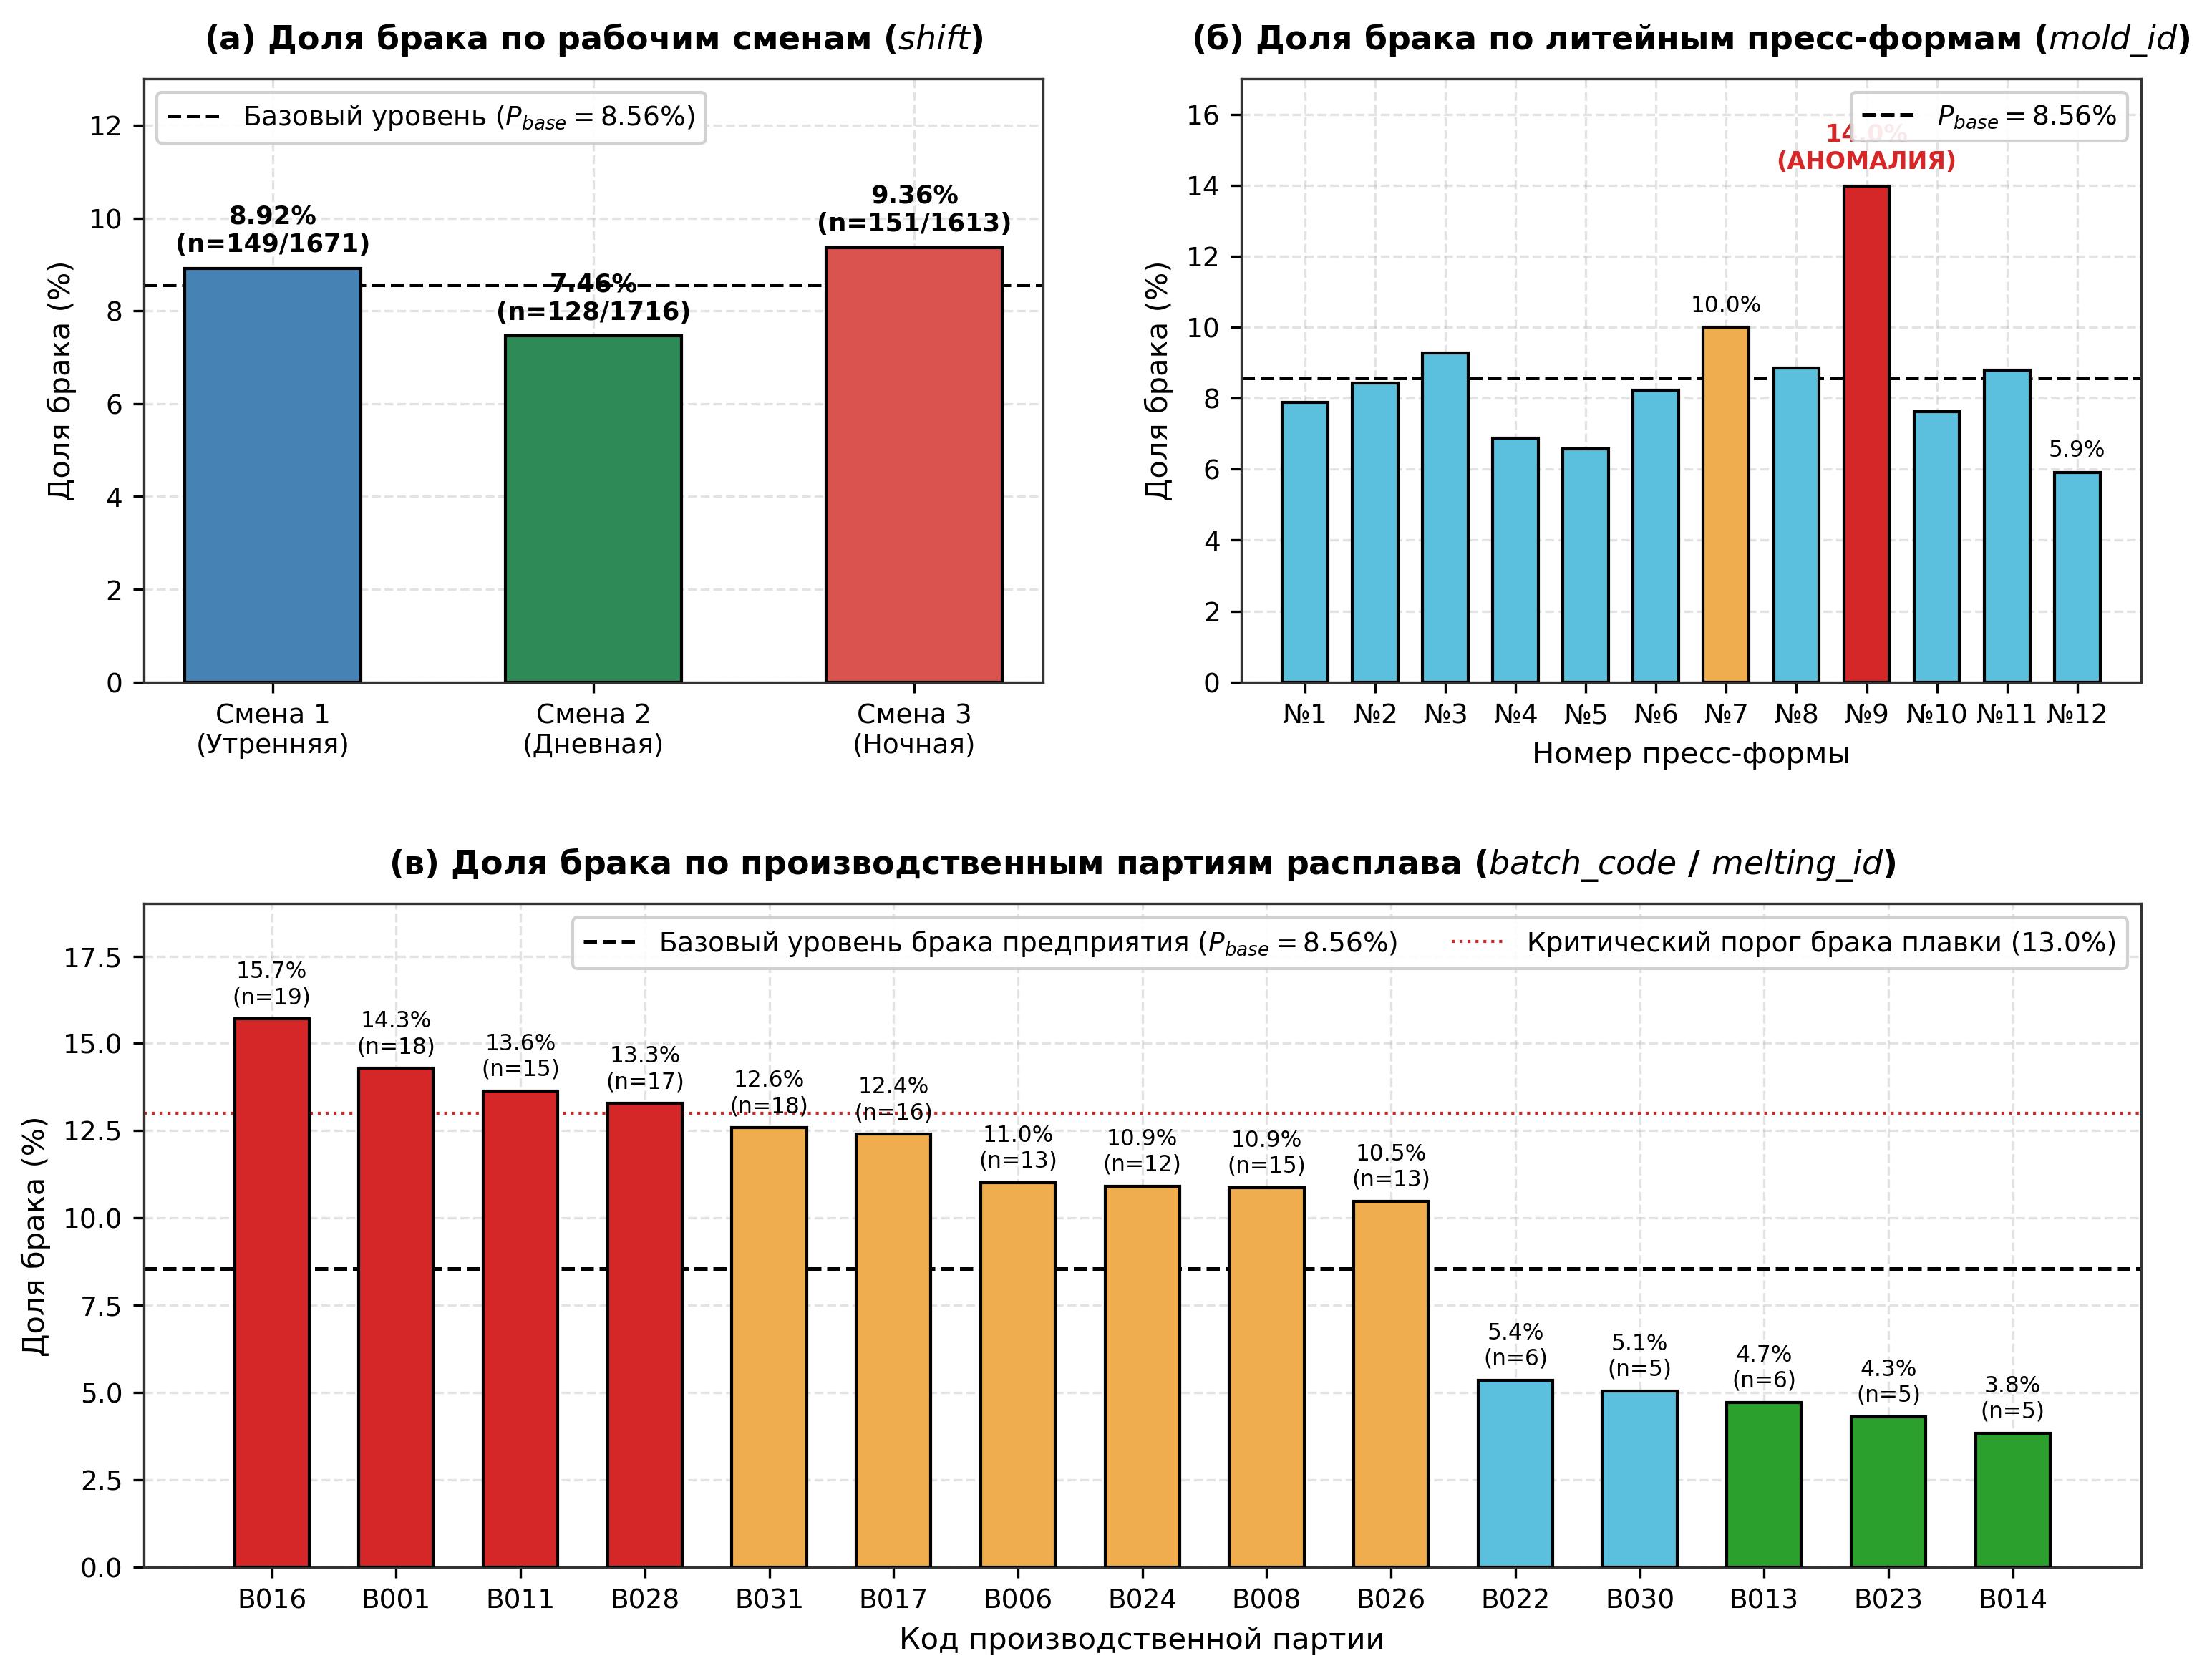
\includegraphics[width=0.85\linewidth]{pictures/fig1_bar_shift_batch.png}
		\caption{Столбчатая диаграмма распределения брака по сменным факторам и оснастке}
	\end{figure}

	\begin{figure}[!h]
		\centering
		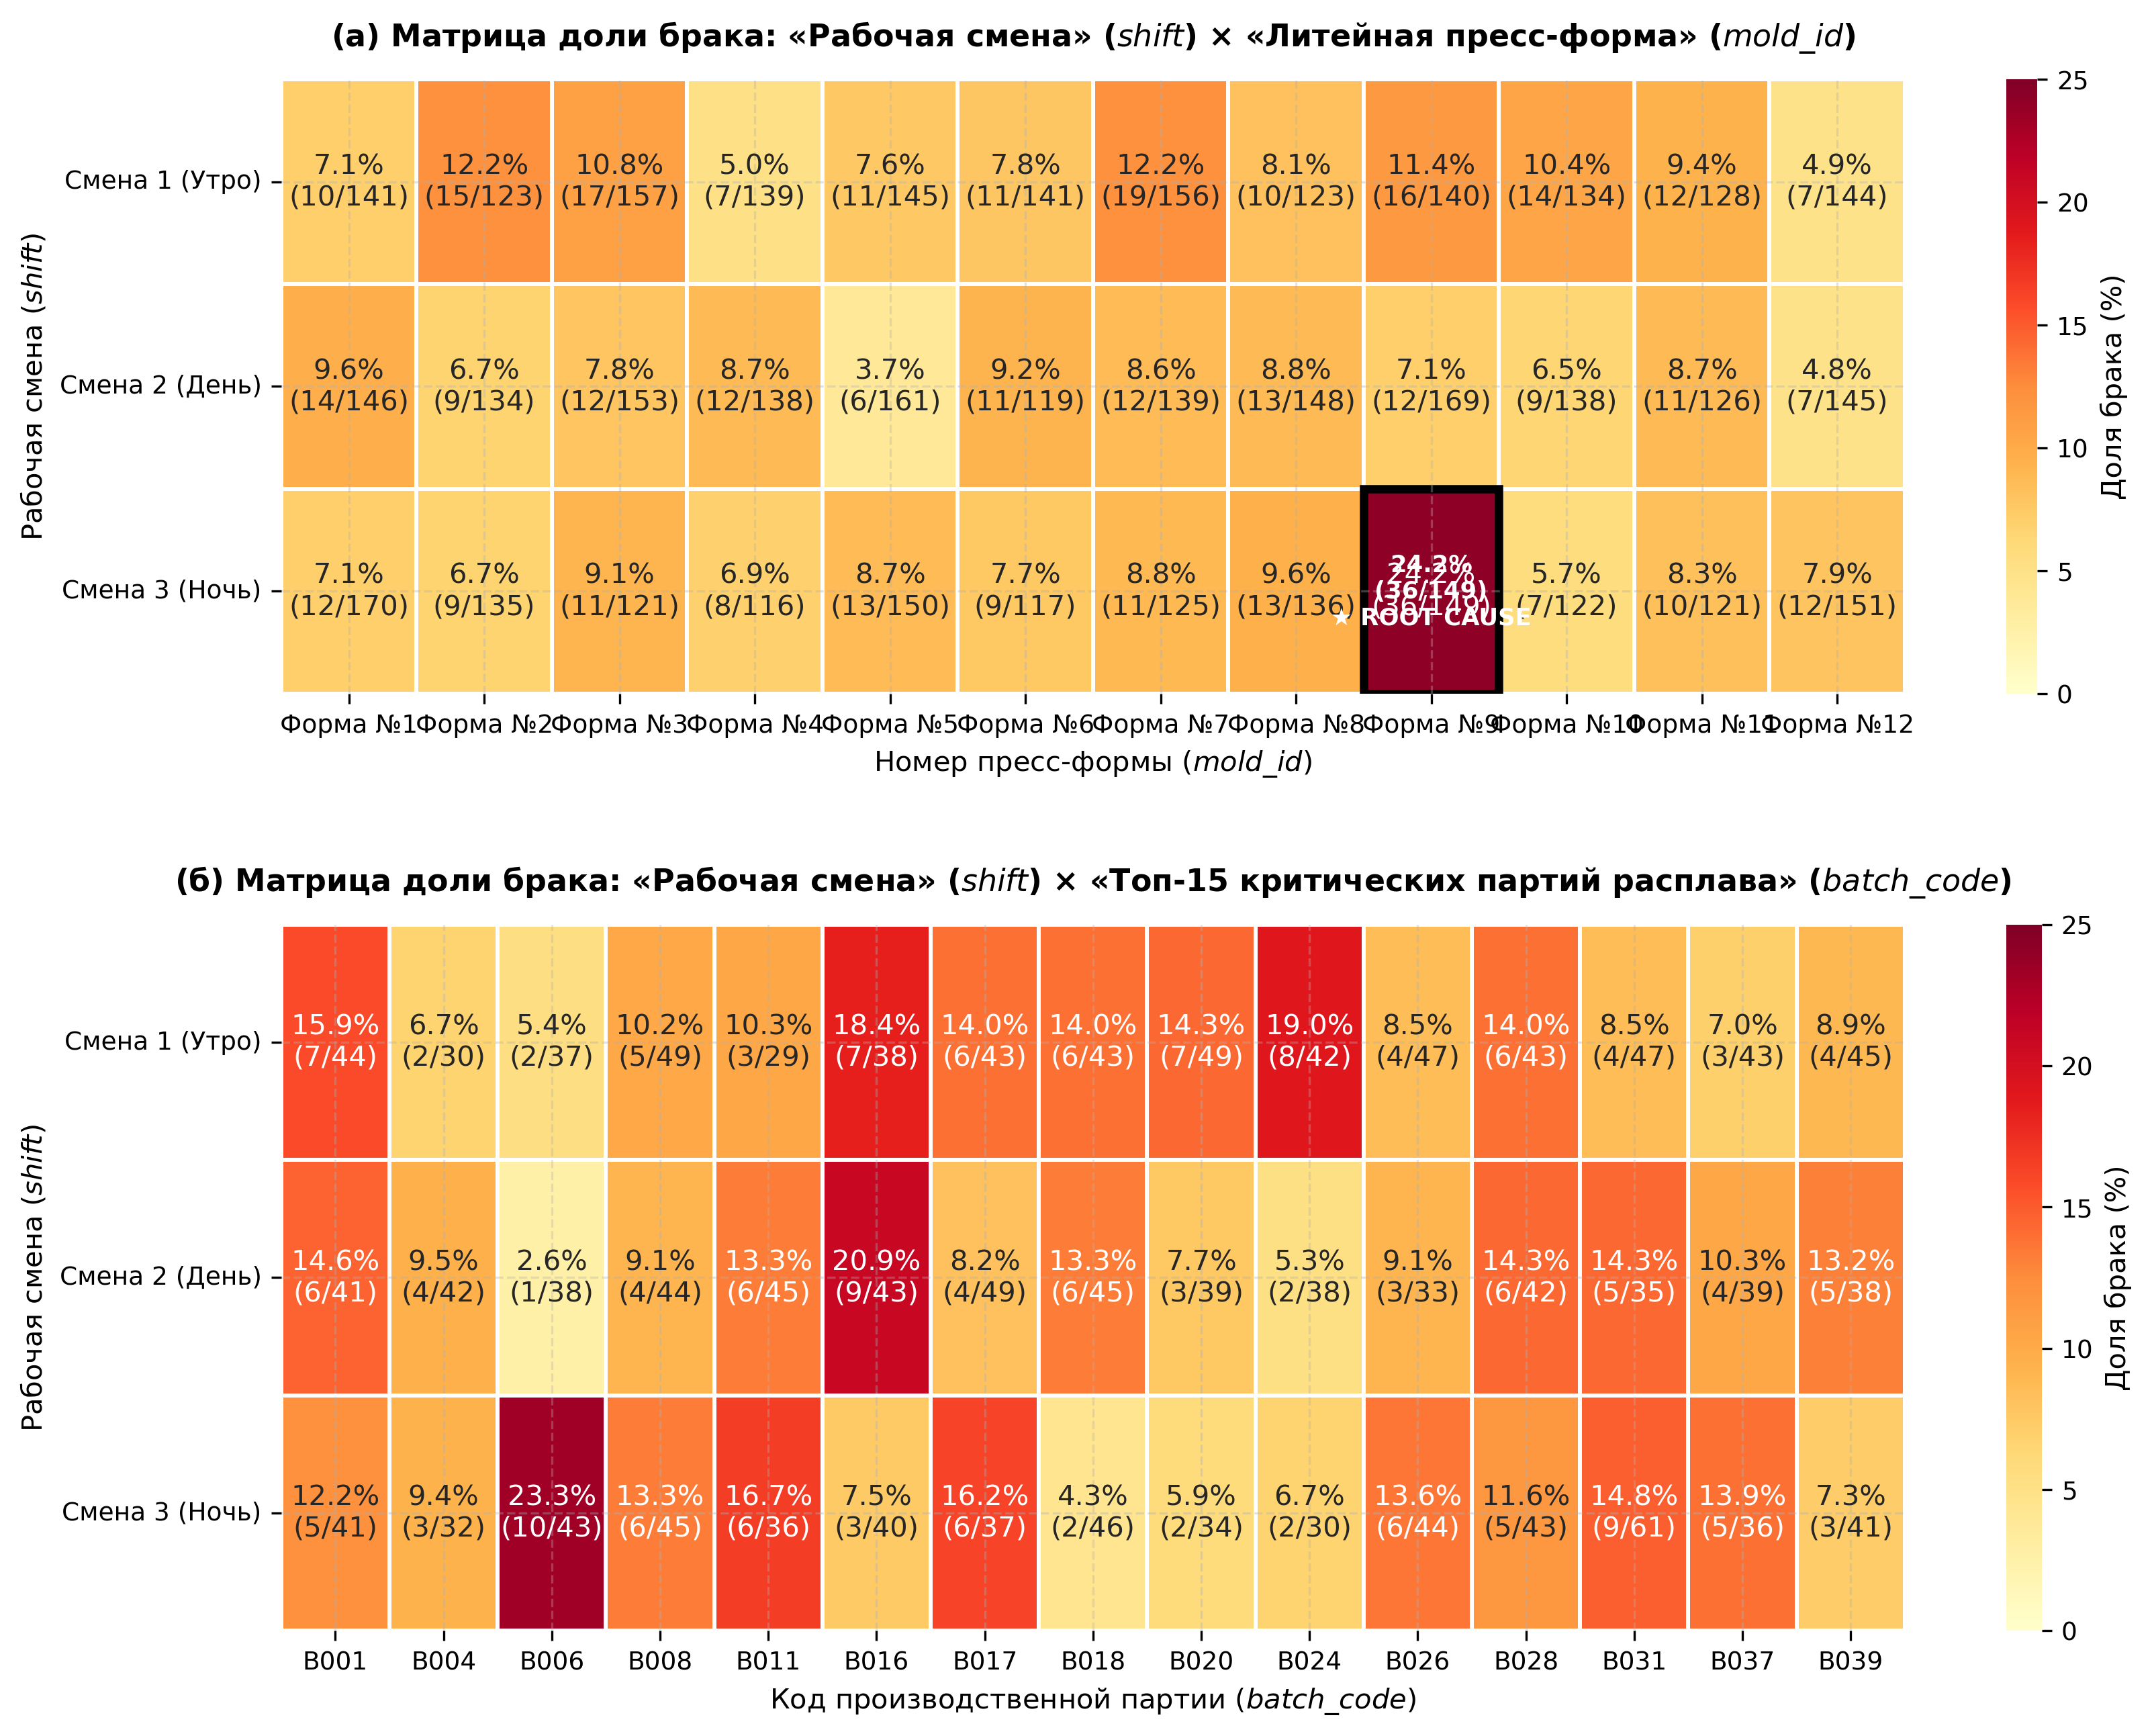
\includegraphics[width=0.85\linewidth]{pictures/fig3_heatmap_categorical_interactions.png}
		\caption{Тепловая карта риска брака в координатах «Смена $\times$ Пресс-форма»}
	\end{figure}

	\section{Анализ технологических параметров в проблемной группе}
	Сравнение выборок проблемной группы {\text{prob}} = \{\text{Смена 3} \times \text{Форма 9}\}$ с остальным массивом выявило комплекс из 4 одновременных критических сдвигов режима (критерий Уэлча  < 10^{-15}$, величина эффекта Коэна $|d| > 1{,}2$):
	\begin{enumerate}
		\item Перегрев расплава при заливке: $+13{,}65^\circ ( = +1{,}30$);
		\item Деградация охлаждения формы № 9: $-40{,}93\%$ ( = -1{,}29$);
		\item Избыточная ковшевая выдержка: $+34{,}75\%$ ( = +2{,}52$);
		\item Рост растворенных газов (водорода): $+24{,}57\%$ ( = +1{,}33$).
	\end{enumerate}

	\begin{figure}[!h]
		\centering
		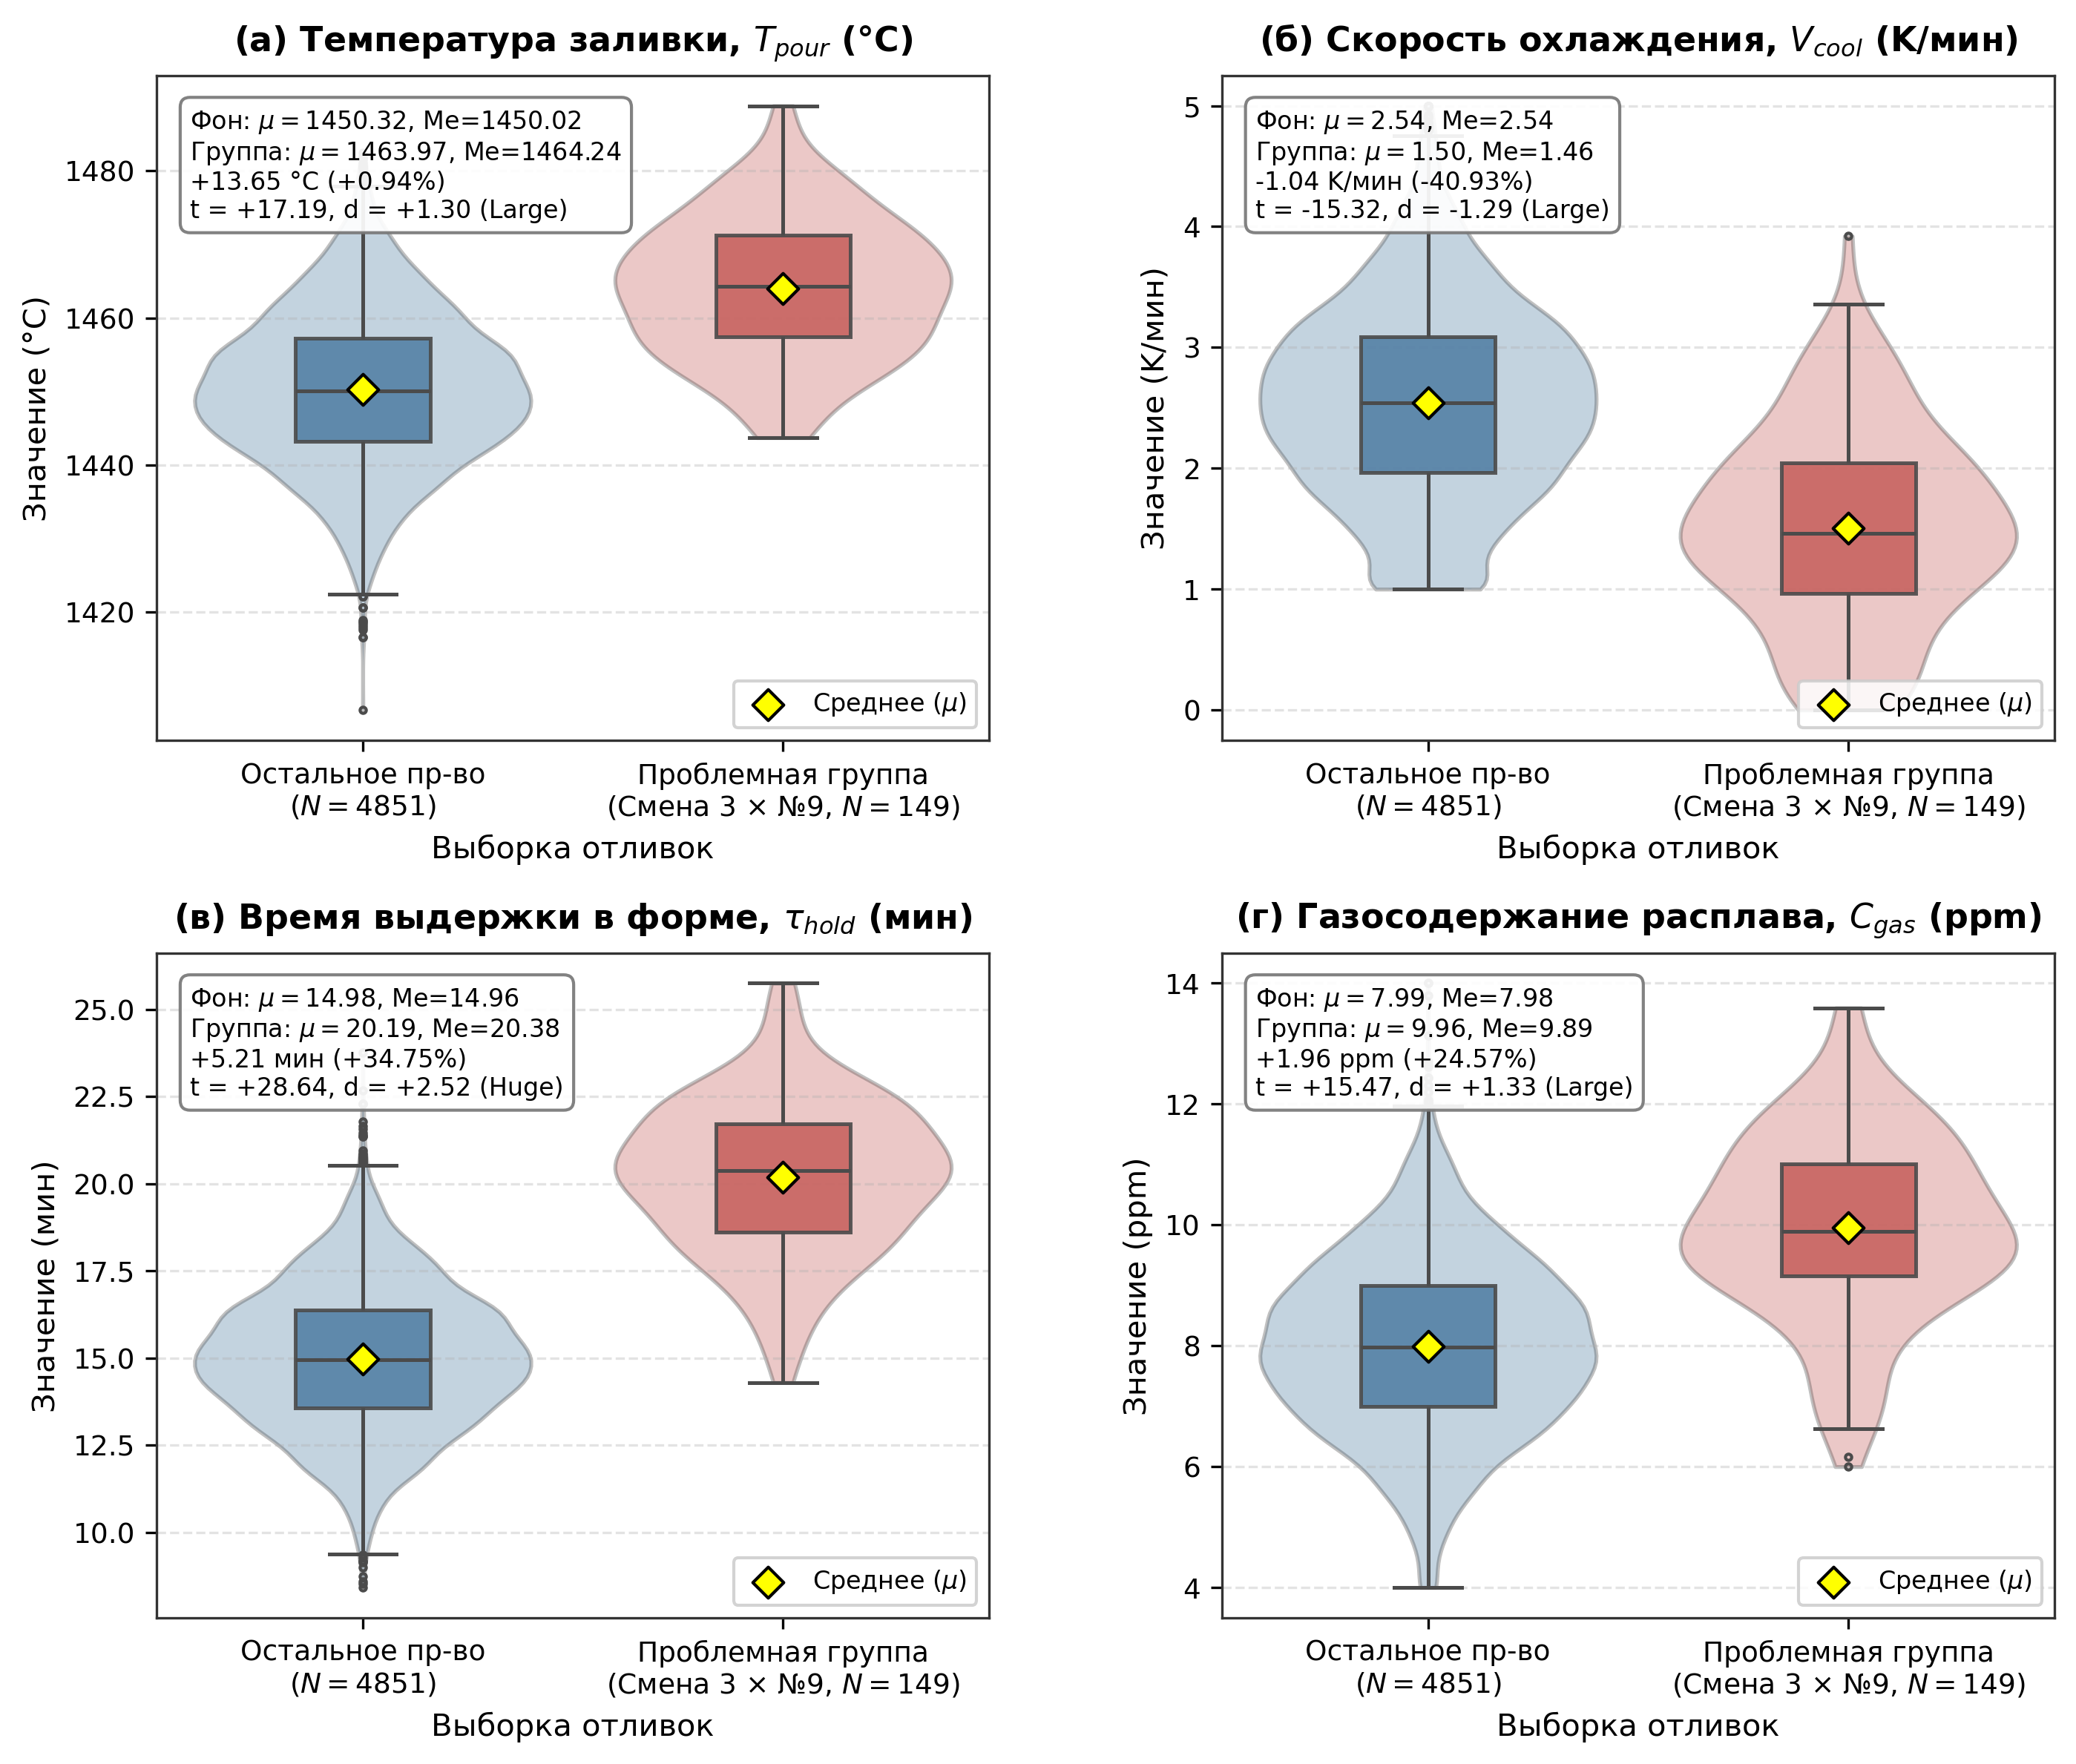
\includegraphics[width=0.85\linewidth]{pictures/fig4_technological_parameters_comparison.png}
		\caption{Сравнение технологических параметров в проблемной группе и вне ее}
	\end{figure}

	\section{Выводы и инженерные рекомендации}
	\begin{enumerate}
		\item Локализован скрытый очаг системного брака, обусловленный синергетическим наложением человеческого фактора ночной смены и тепловой деградации каналов охлаждения пресс-формы № 9.
		\item Внедрение превентивного алгоритма раннего предупреждения (EWS) на основе дистанции Махаланобиса обеспечивает снижение брака на {,}5$--{,}0\%$ в абсолютном выражении.
	\end{enumerate}

	\section{Литература}
	\begin{enumerate}
		\item Мосин В. Г., Козловский В. Н. Повышение производительности регрессионных моделей при оценке качества потребления электронного контента // Известия ТулГУ. Технические науки. 2024. № 2. С. 593--599.
		\item Мосин В. Г., Козловский В. Н., Васин С. А., Стрелков Г. С. Мониторинг данных о результативности процессов системы менеджмента // Известия ТулГУ. Технические науки. 2024. № 4. С. 28--33.
		\item Козловский В. Н., Антипова О. И. Комплекс методов управления качеством автомобильной продукции // Стандарты и качество. 2023. № 8. С. 42--46.
		\item Монтгомери Д. Статистический контроль качества. — М.: Вильямс, 2017. — 848 с.
	\end{enumerate}
\end{document}
